\section{Solver Parameter Testing}

\begin{frame}{Solver Parameter Testing}
\begin{itemize}
\item Certain parameters can be varied during the modeling of detonations 
\item Plots shown are pressure distributions, which agree in regards to convergence to temperature and velocity distribution plots
\item Grid resolutions will be referred to as their number of cells in that dimension, or primarily in tube length which is 0.25 m long. 
\end{itemize}
\end{frame}

\subsection{Detonation Ignition Testing}

\begin{frame}{Ignition Tests}
\begin{itemize}
\item Detonations can be initialized several ways
\begin{itemize}
    \item high $T$ and $P$ reactant block
    \item high $T$ and $P$ inert (e.g. helium) block
    \item gradient ignition, shown by Towery \textit{et. al.} \cite{towery2}
\end{itemize}
\item Necessary to test before AMR testing began 
\end{itemize}    
\end{frame}

\begin{frame}{Block Ignition}
Block of reactants at 3000 K and 20 atm spanning 0.001 m:
\begin{figure}[]
\centering
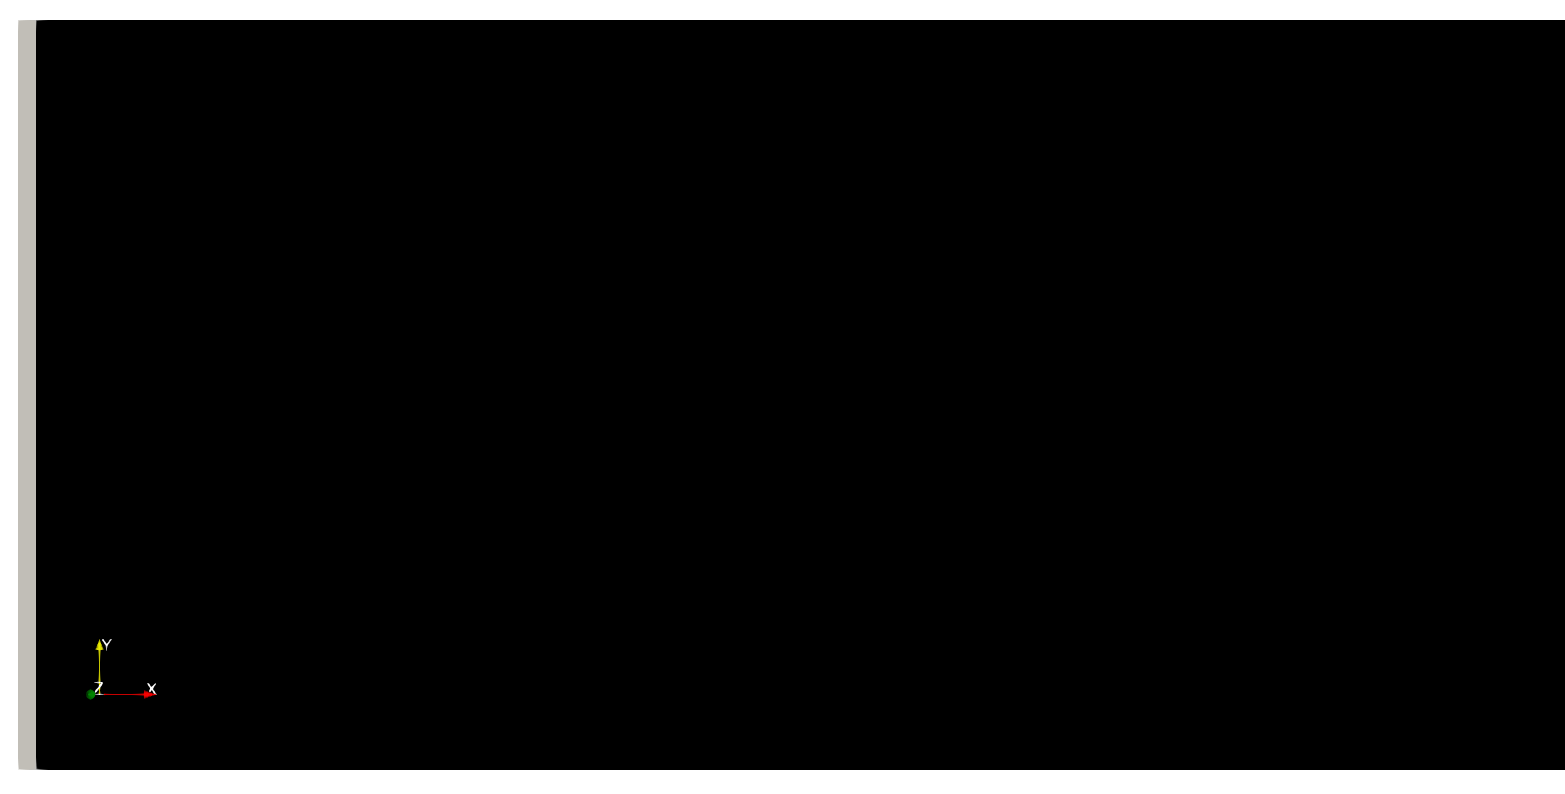
\includegraphics[width=0.7\textwidth]{../figs/ignition/block.png}
%\caption{Block ignition method, seen on left side of domain, at t = 0 s}
%\label{fig:blockig}
\end{figure}%
Abandoned due to due instability in detonation initiation.
\end{frame}

\begin{frame}{Gradient Ignition}
Gradient spanning from 1200 K and 4 atm to 300 K and 1 atm over 0.01 m:
\begin{figure}[]
\centering
\includegraphics[width=0.7\textwidth]{../figs/ignition/gradient.png}
%\caption{Block ignition method, seen on left side of domain, at t = 0 s}
%\label{fig:blockig}
\end{figure}%
This produced smoother and more consistent detonations. 
\end{frame}


\subsection{Arrhenius Pre-exponential Factor Variation}

\begin{frame}{Arrhenius Pre-exponential Factor $A$ Variation}
\begin{itemize}
\item Wanted to gauge sensitivity to Arrhenius pre-exponential factor as well as get a sense of how values compare to published values
\item Swept exponent between $10^{11}$ and $10^{17}$ 
\item Plotted CJ target from similar setup by Towery \textit{et. al.} \cite{towery1}
\end{itemize}
\end{frame}

\begin{frame}{Arrhenius $A$ Variation: Pressure Distribution}
\begin{figure}
\centering
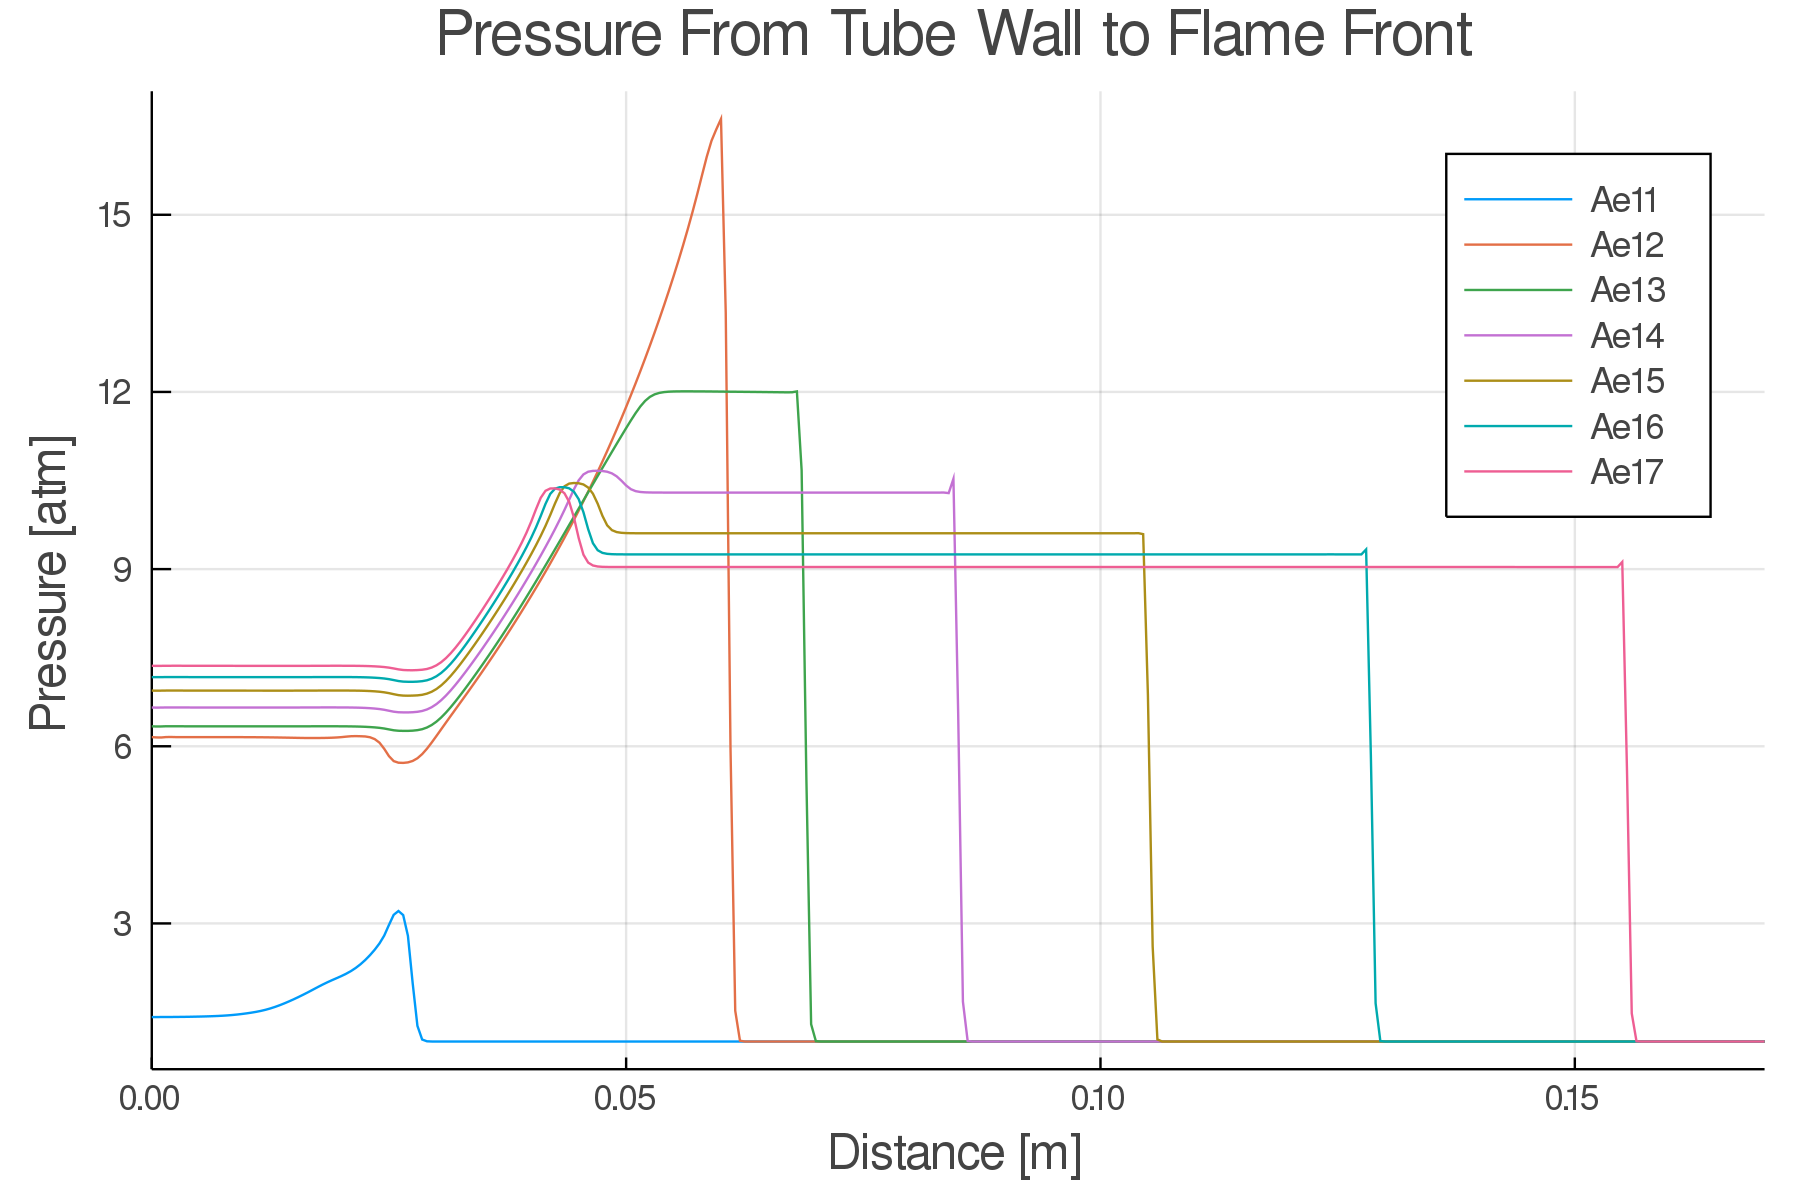
\includegraphics[width=0.8\linewidth]{../figs/Atest/p.png}
%\caption{Pressure distribution in detonation tube for pre-exponential factor exponent sweep test}
%\label{fig:atestp}
\end{figure}
\end{frame}

\begin{frame}{Arrhenius $A$ Variation: Detonation Decoupling}
\begin{figure}
\centering
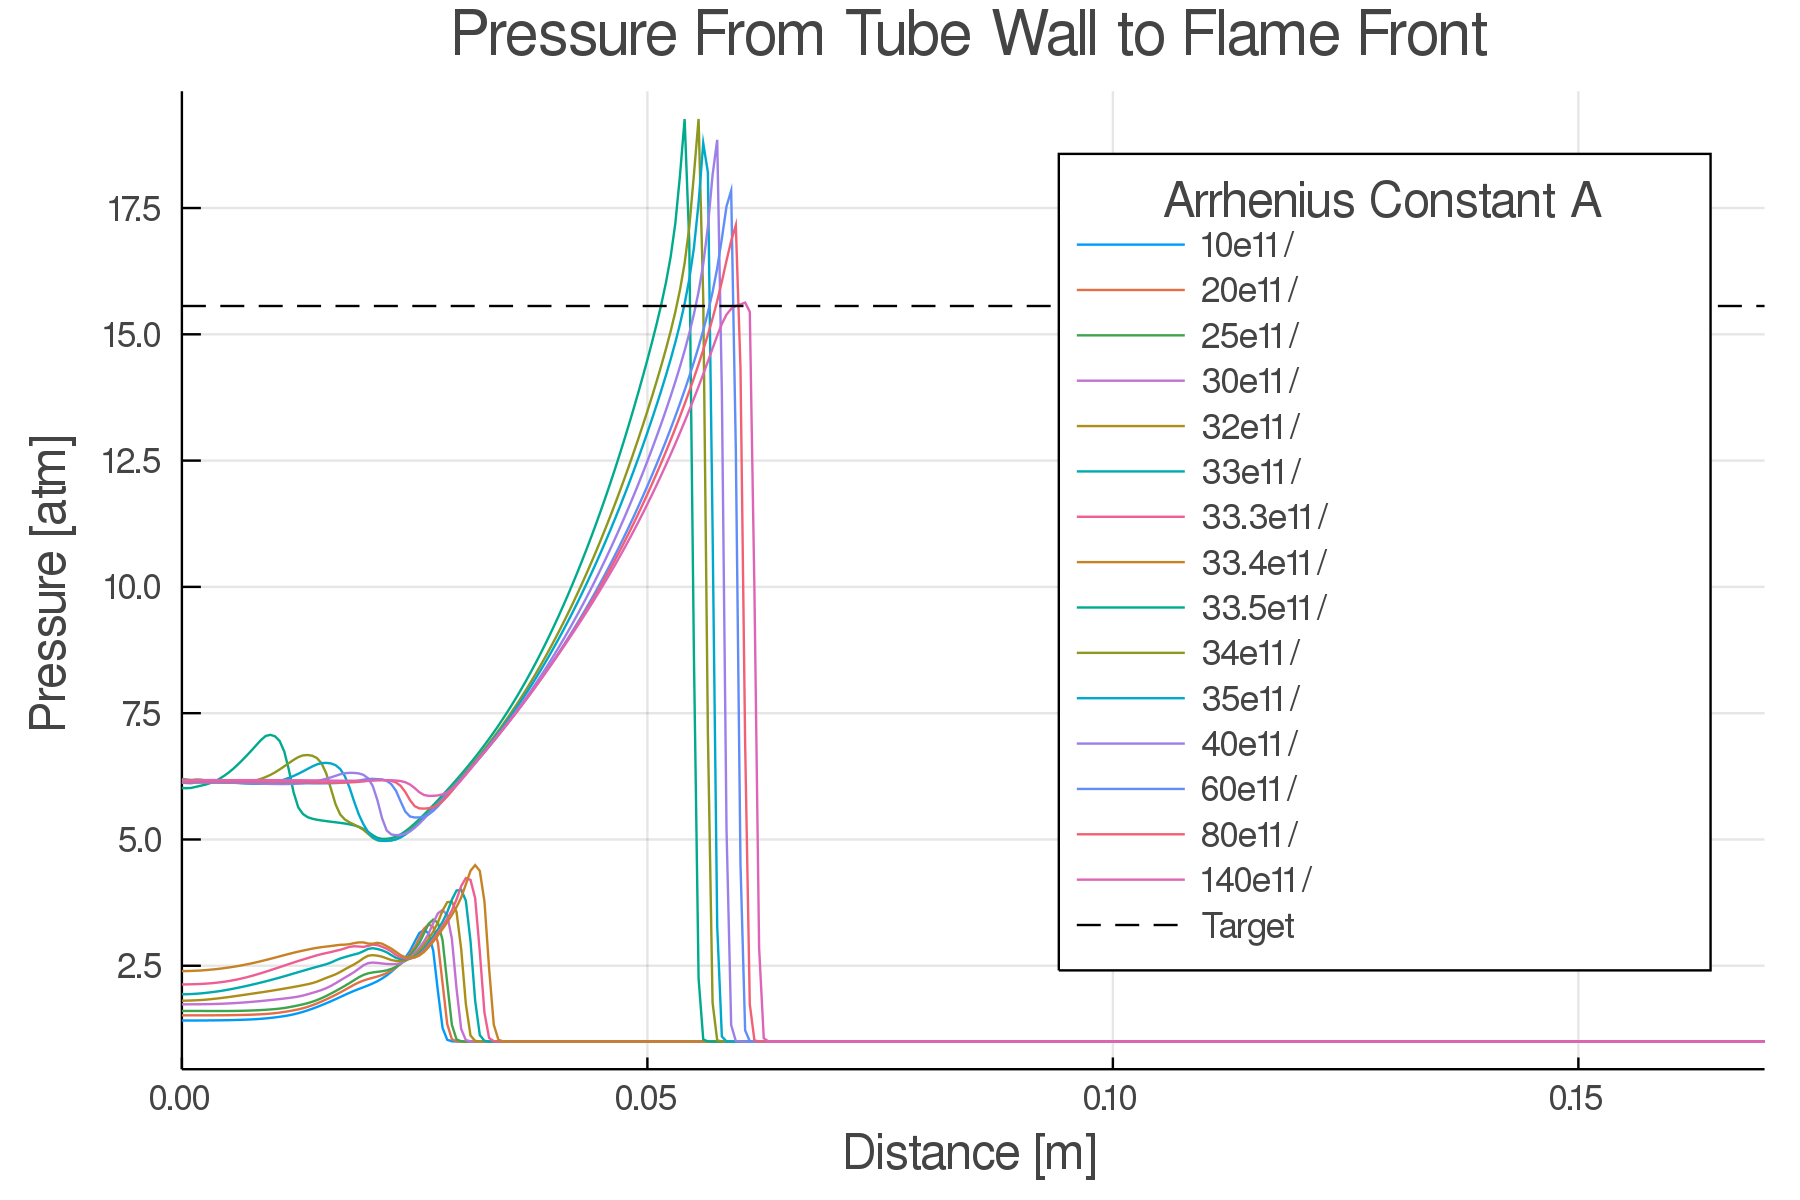
\includegraphics[width=0.8\linewidth]{../figs/Atest_refined/p_large.png}
%\caption{Pressure distribution in detonation tube for expanded and refined pre-exponential factor exponent sweep test, showing detonation shock-reaction coupling transition. See Figures \ref{fig:atestrp} and \ref{fig:atestrt} for a filtered version.}
%\label{fig:pjump}
\end{figure}
\end{frame}

\subsection{Time Step Variation}

\begin{frame}{Time Step Variation}
\begin{itemize}
\item Larger timesteps reduce computational expense, but can increase solution instability
\item \texttt{rhoReactingCentralFoam} can change timestep based on both max-desired central and acoustic Courant numbers
\begin{itemize}
    \item most existing OpenFOAM solvers track solely the central courant number
\end{itemize}
\item To characterize solution behavior, the max-allowed CFL was varied 
\end{itemize}
\begin{table}[]
\centering
%\caption{Max CFL errors compared to CFL = 0.01}
%\label{tab:cflerror}
\begin{tabular}{cccc}
Max CFL & Pressure Error (\%) & Temperature Error (\%) & Velocity Error (\%) \\ \hline
0.3 & 57.18 & 19.54 & 27.62 \\ 
0.2 & 5.89 & 8.72 & 8.66 \\
0.1 & 1.28 & 2.71 & 12.92 \\
0.05 & 2.34 & 1.29 & 8.96 \\
0.01 & 0 & 0 & 0 \\
\end{tabular}
\end{table}% 
\end{frame}

\begin{frame}{Time Step Variation: Pressure Distribution}
\begin{center}
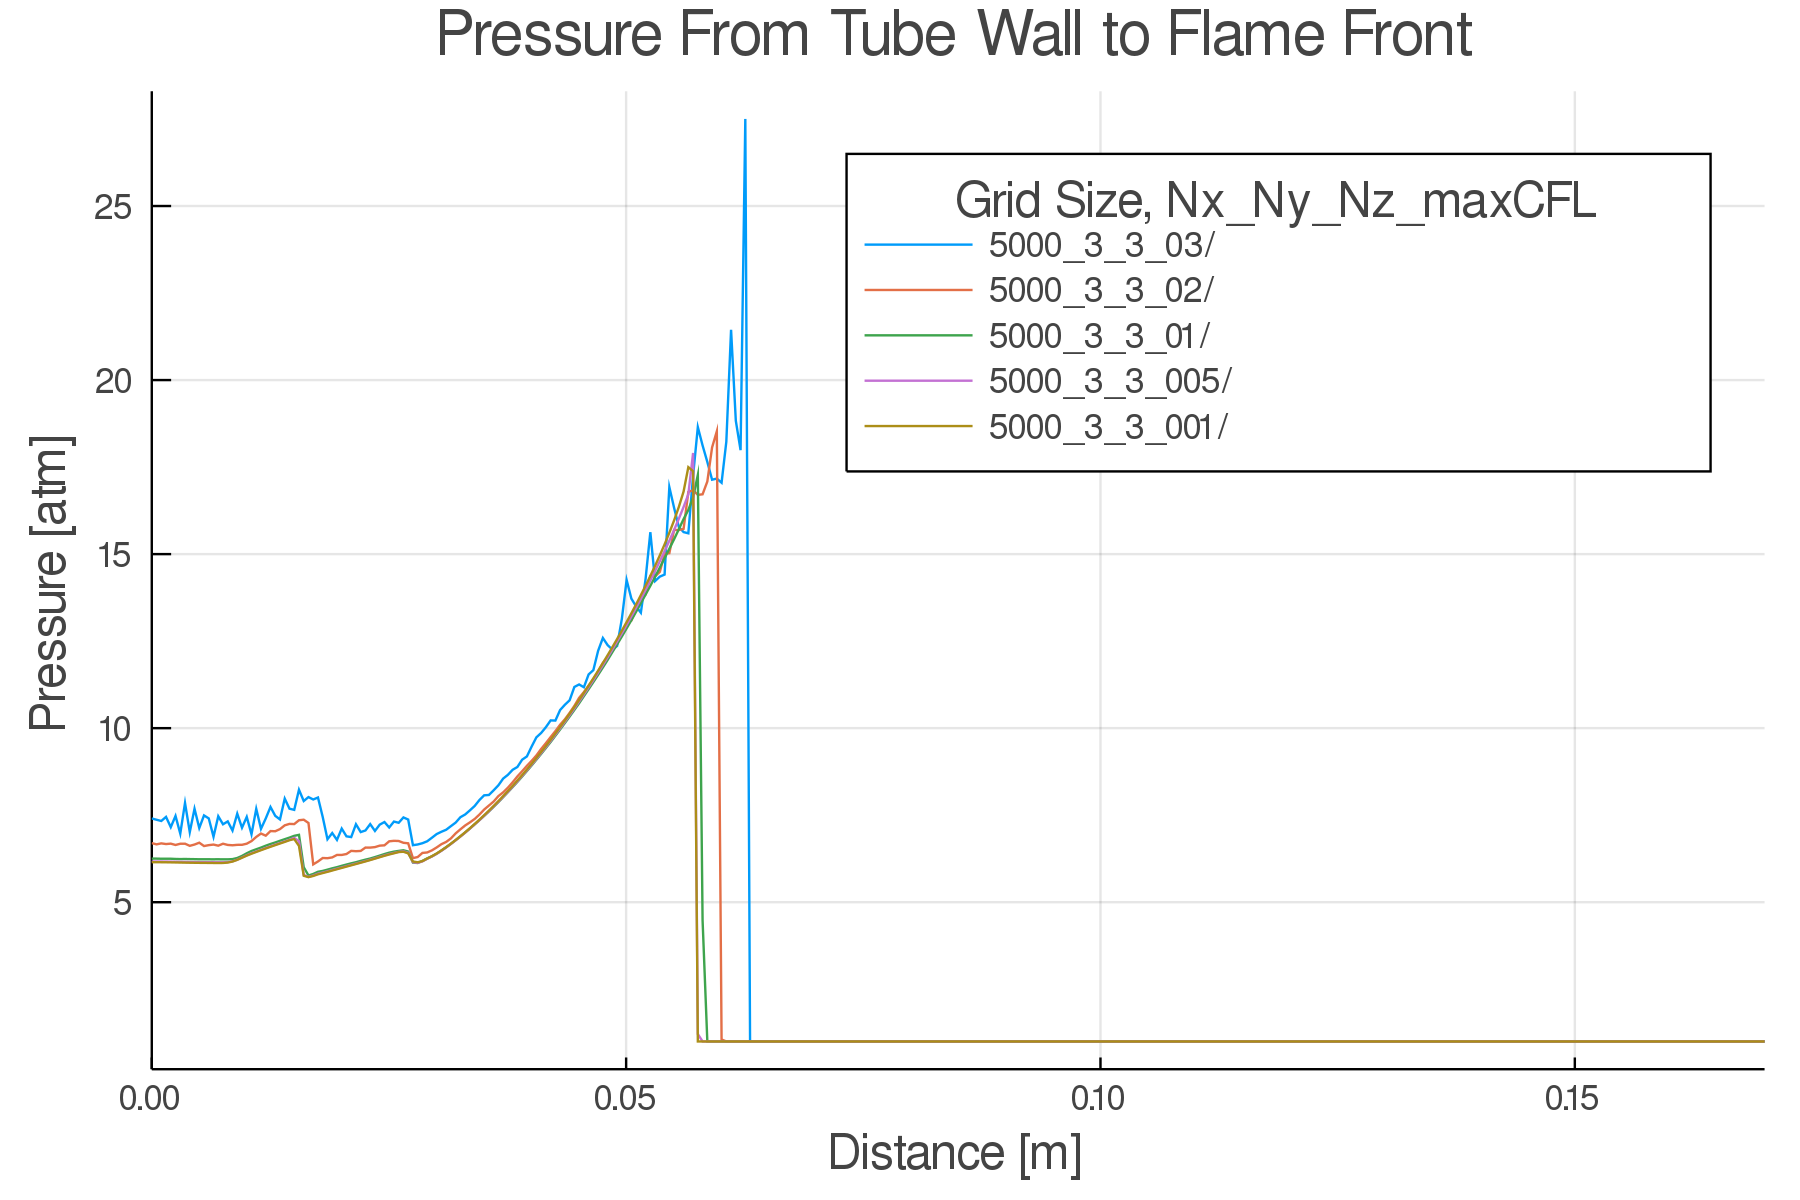
\includegraphics[width=0.8\textwidth]{../figs/cfl_test/p.png}
\end{center}
\end{frame}

\subsection{Static Mesh Variation}

\begin{frame}{Static Mesh Variation}
\begin{itemize}
\item Before comparing AMR, need to have baseline static meshes 
\item Start with one-dimensional, move to two-dimensional 
\item Static mesh resolutions will help determine convergence criteria for:
\begin{itemize}
    \item overall detonation shape convergence 
    \item ZND Von Neumann pressure spike convergence 
    \item fine detonation structure convergence
\end{itemize}
\end{itemize}
\end{frame}

\begin{frame}{1D Static Mesh Variation: Pressure Distribution}
\begin{center}
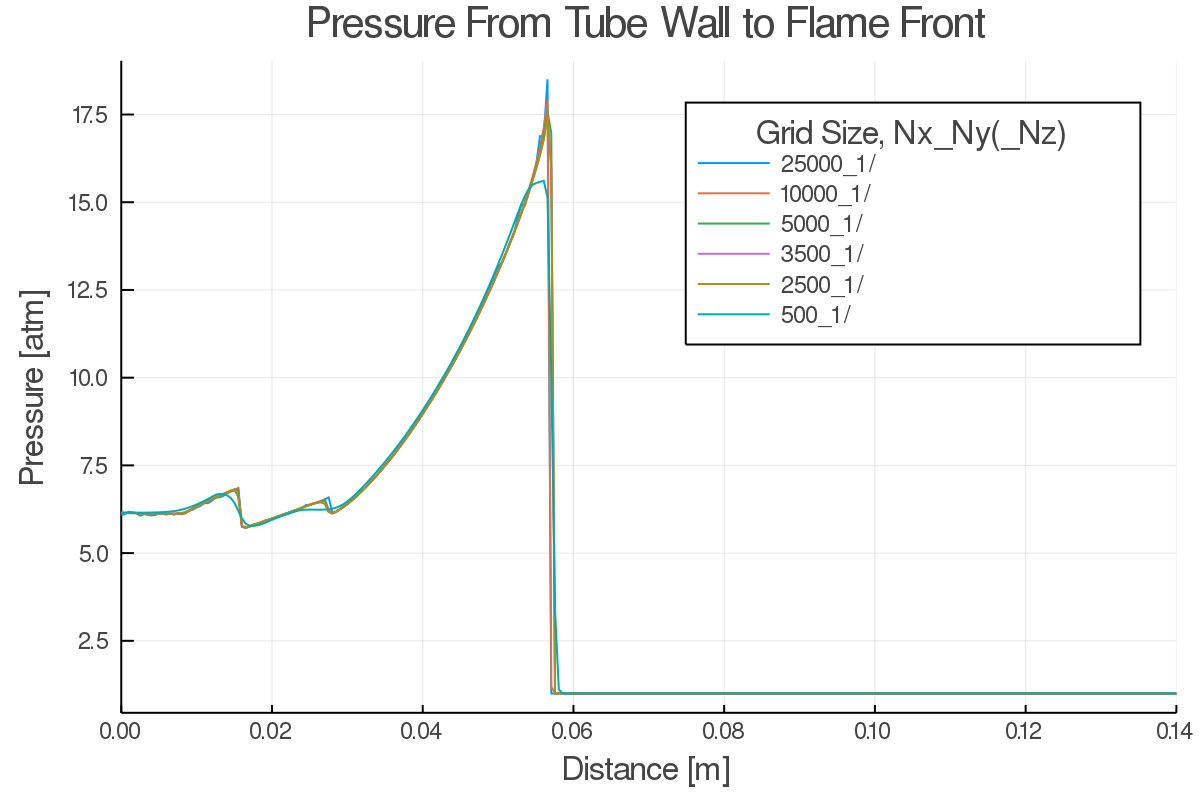
\includegraphics[width=0.8\textwidth]{../figs/static1d/p.png}
\end{center}
\end{frame}

\begin{frame}{2D Static Mesh Variation: Pressure Distribution}
\begin{center}
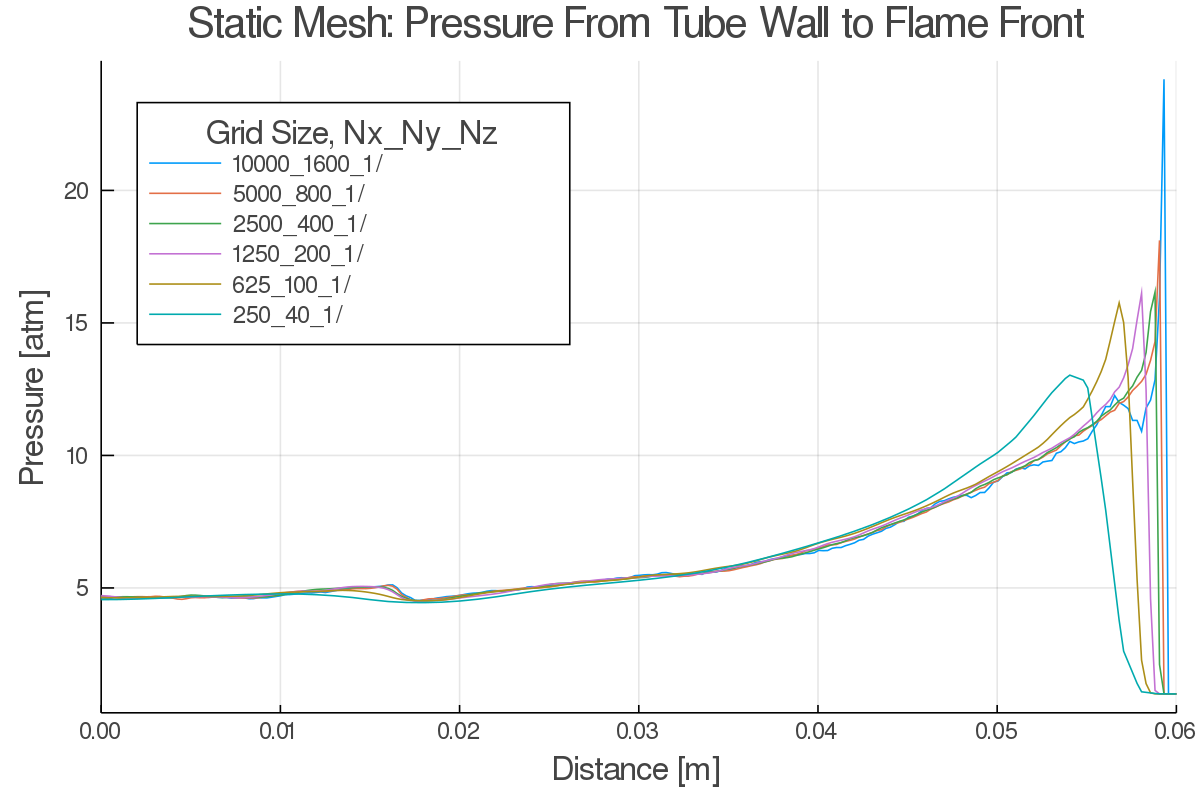
\includegraphics[width=0.8\textwidth]{../figs/staticfigs/p.png}
\end{center}
\end{frame}

\subsection{Adaptive Meshing}

\begin{frame}{Adaptive Mesh Variation and Comparison}
Some AMR comparisons and parameter variations were made next, namely:
\begin{itemize}
\item AMR compared to static meshes
\item AMR refinement level variation
\item AMR buffer layer variation
\item AMR normalized pressure gradient bound variation 
\end{itemize}
\end{frame}

\subsection{AMR and Static Mesh Comparison}

\begin{frame}{AMR vs. Static: Pressure Distribution}
\begin{center}
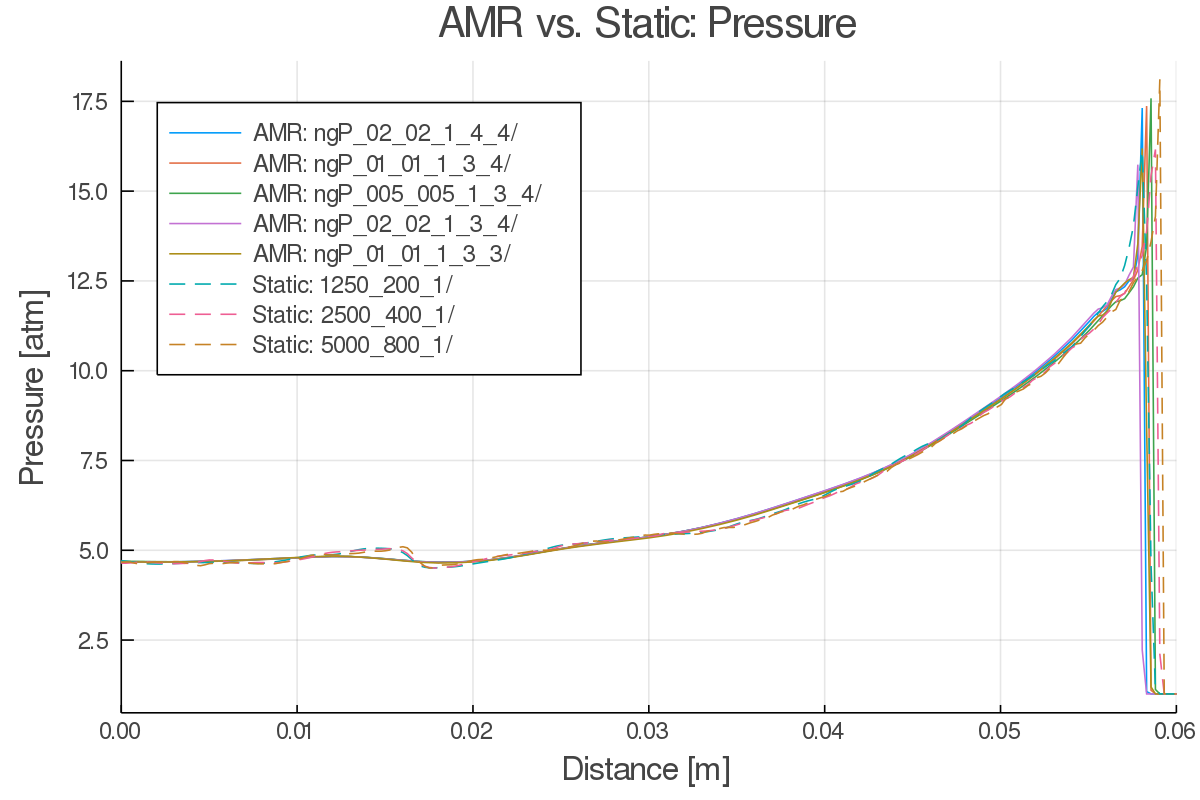
\includegraphics[width=0.8\textwidth]{../figs/amrfigs/amrcompare/p.png}
\end{center}
\end{frame}

\begin{frame}{AMR vs. Static: Pressure Distribution (enlarged)}
\begin{center}
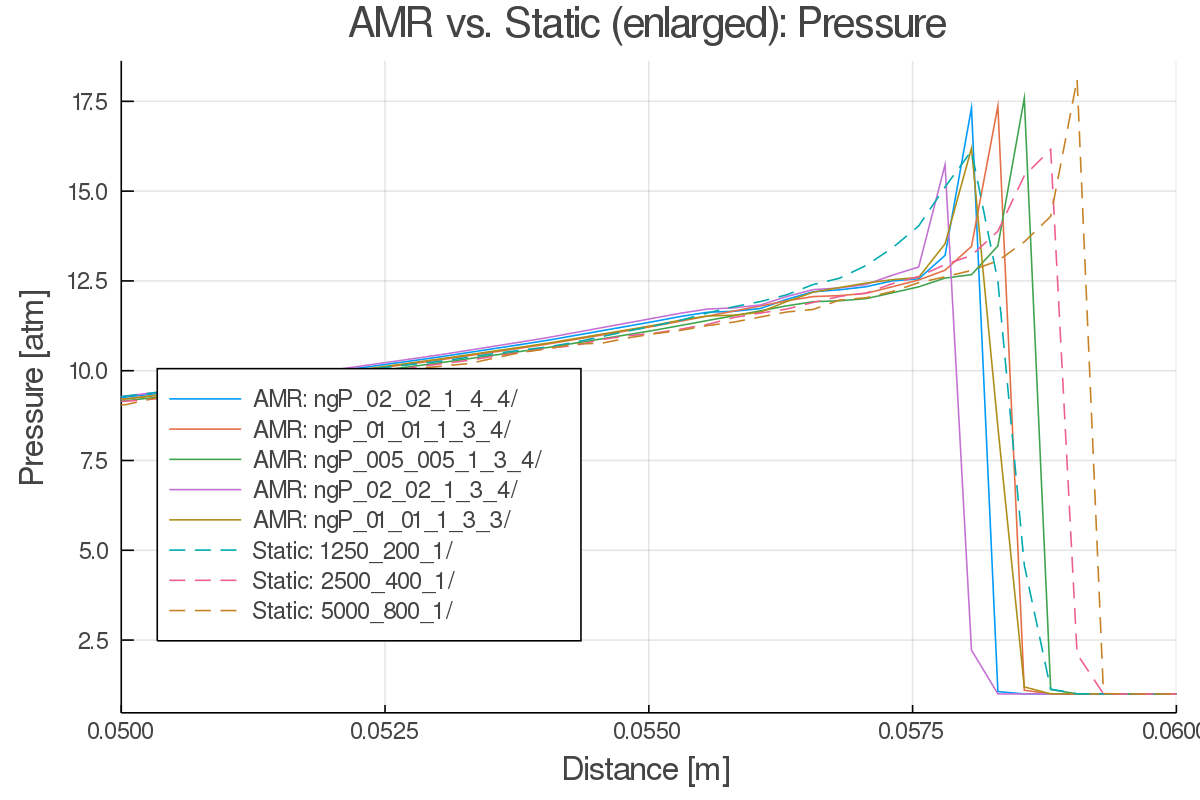
\includegraphics[width=0.8\textwidth]{../figs/amrfigs/amrcompare/pe.png}
\end{center}
\end{frame}

\begin{frame}{AMR and Static Mesh Comparison: Summary}
\begin{itemize}
\item 240-40-1 base mesh, AMR tracking $|| \nabla (p)|| $
\item Good agreement between 1250-200-1 static mesh and AMR with low/unrefine bound of 0.1 and 3 refine and buffer layers; 85\% cell count reduction with exact peak solution reproduction
\item AMR with low/unrefine bound of 0.2 and 4 refine and buffer layers can model peak conditions of 5000-800-1 mesh with 96\% reduction in cell count ($\Delta x \approx 0.00125 $ m)
\item Interesting observation: purple AMR run has more refinement levels than brown but brown has a lower AMR trigger bound and is more accurate overall, while being 3.8x smaller
\end{itemize}
\end{frame}

\begin{frame}{AMR and Static Mesh Comparison: Summary ii}
Type colors match static targets to AMR:
\begin{table}[]
\scalebox{0.9}{
\centering
%\caption{AMR and Static Mesh Cell Count Comparisons for Figure \ref{fig:amrcompare}, tracking normalized pressure gradient}
%\label{tab:amrcompare}
\begin{tabular}{ccp{2cm}p{2cm}p{2cm}p{2cm}c}
Mesh & Type & Unrefine/ lowrefine & Upper ~~~ refine & Buffer ~~ layers & Refine ~~ levels& Cell Count \\ \hline \hline
1250-200-1 & {\color{blue}Static} & - & - & - & - & 250,000 \\ 
2500-400-1 & Static & - & - & - & - & 1,000,000 \\
5000-800-1 & {\color{red}Static} & - & - & - & - & 4,000,000 \\ \hline
250-40-1 & {\color{red}AMR} & 0.2 & 1 & 4 & 4 & 148,950 \\
250-40-1 & {\color{red}AMR} & 0.1 & 1 & 3 & 4 & 149,762 \\
250-40-1 & {\color{red}AMR} & 0.05 & 1 & 3 & 4 & 160,570 \\ \hline
250-40-1 & {\color{blue}AMR} & 0.2 & 1 & 3 & 4 & 146,710 \\ 
250-40-1 & {\color{blue}AMR} & 0.1 & 1 & 3 & 3 & 38,343 \\ 
\end{tabular}
}
\end{table}
\end{frame}

\subsection{AMR Refinement Level Variation}

\begin{frame}{AMR Refinement Level Variation: Pressure Distribution}
\begin{center}
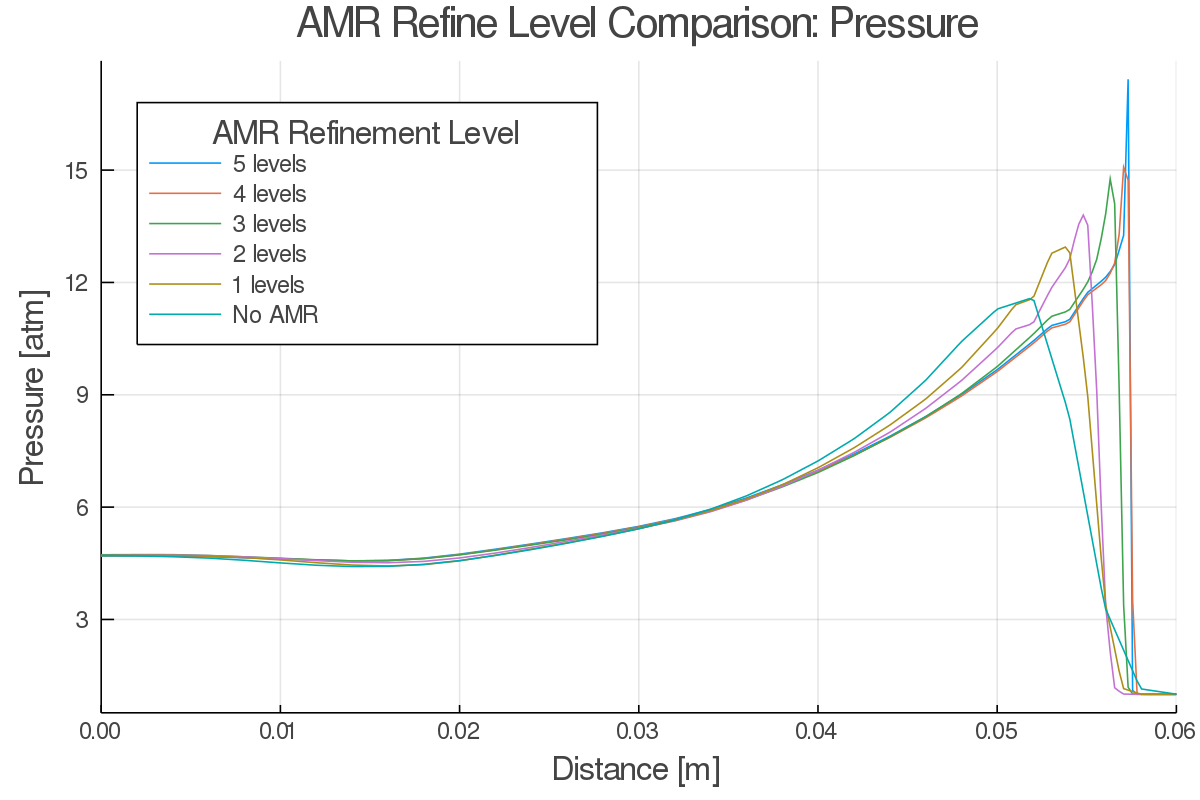
\includegraphics[width=0.8\textwidth]{../figs/amrfigs/amr_refinelevels/p.png}
\end{center}
\end{frame}

\begin{frame}{AMR Refinement Level Variation: Pressure Distribution (enlarged)}
\begin{center}
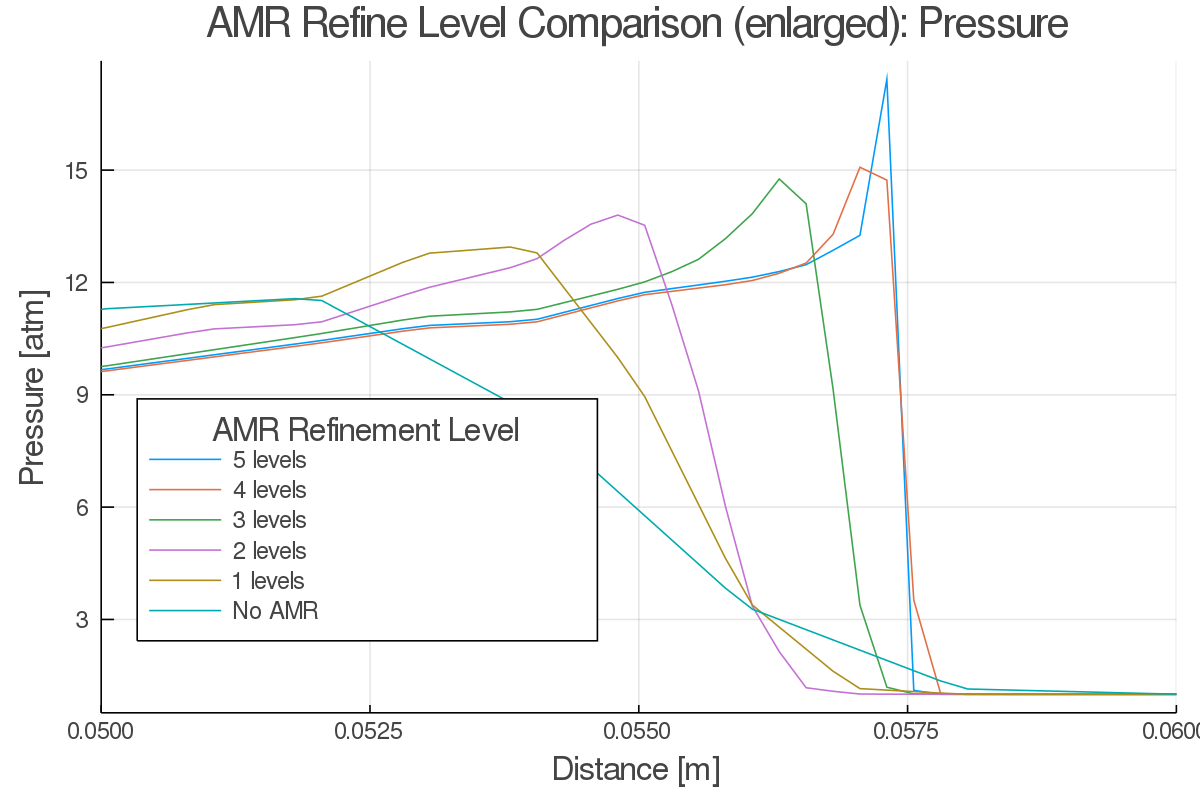
\includegraphics[width=0.8\textwidth]{../figs/amrfigs/amr_refinelevels/pe.png}
\end{center}
\end{frame}


\begin{frame}{AMR Refinement Level Variation Summary}
\begin{columns}
\column{0.6\textwidth}
\begin{itemize}
\item 125-20-1 base mesh
\item tracking $||\nabla (p)||$ from 0.2 to 1, unrefining below 0.2, with 3 buffer layers
\item 4 levels (2000-320-1) to begin resolving von Neumann spike, agrees with static trends
\item 5 levels nearly matches peak pressure of 5000-800-1 static mesh with 3.7m fewer cells
%\item each level exponentially more computationally expensive 
\item cells scale exponentially with refinement level
\end{itemize}

\column{0.4\textwidth}
\begin{table}[h]
\centering
%\caption{Cells for each refinement level for the 125-20-1 simulation at \(t = 3\times 10^{ - 5} s\) in Figure \ref{fig:amr_refinelevels}}
%\label{tab:amr_refinelevels}
\begin{tabular}{cc}
Refinement Level & Cells \\ \hline
5 & 228,607 \\ 
4 & 54,678 \\ 
3 & 13,028 \\ 
2 & 5,300 \\
1 & 2,920 \\
None & 2500 \\
\end{tabular}
\end{table}
\end{columns}
\end{frame}

\subsection{AMR Buffer Layer Variation}

\begin{frame}{AMR Buffer Layer Variation: Pressure Distribution}
\begin{center}
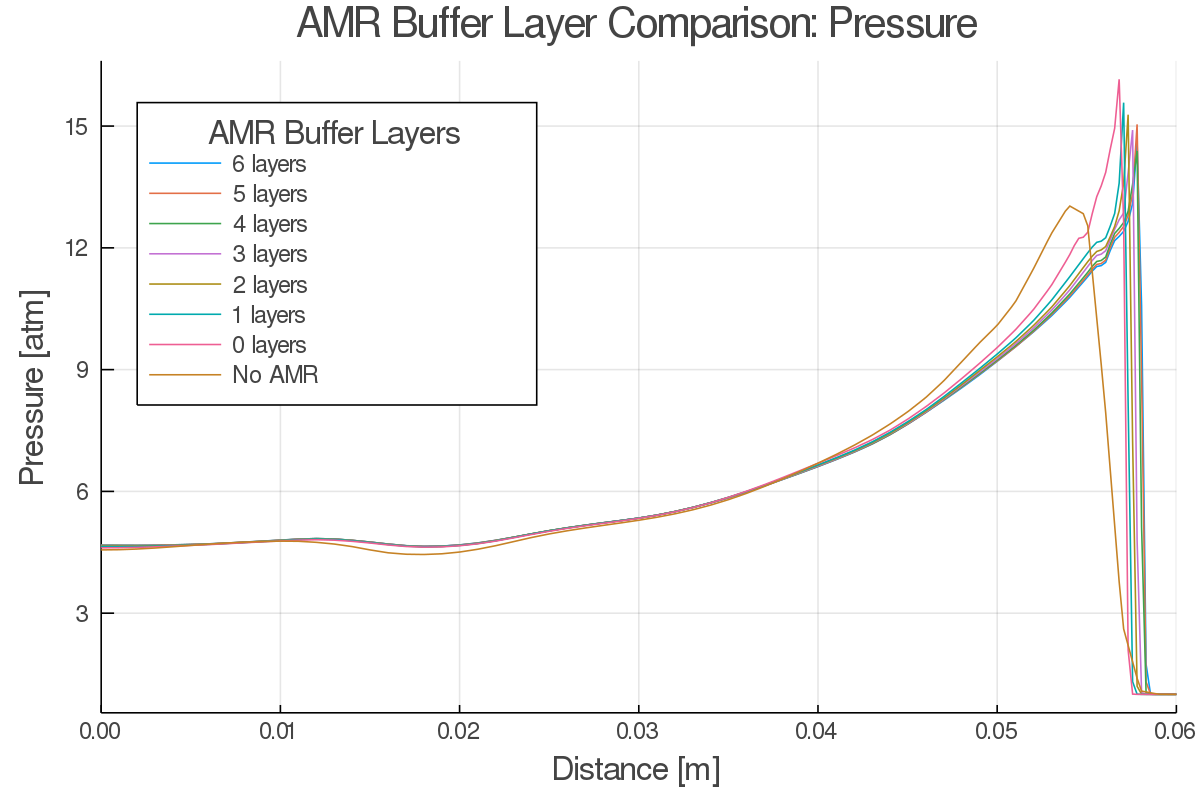
\includegraphics[width=0.8\textwidth]{../figs/amrfigs/amr_bufflayers/p.png}
\end{center}
\end{frame}

\begin{frame}{AMR Buffer Layer Variation: Pressure Distribution (enlarged)}
\begin{center}
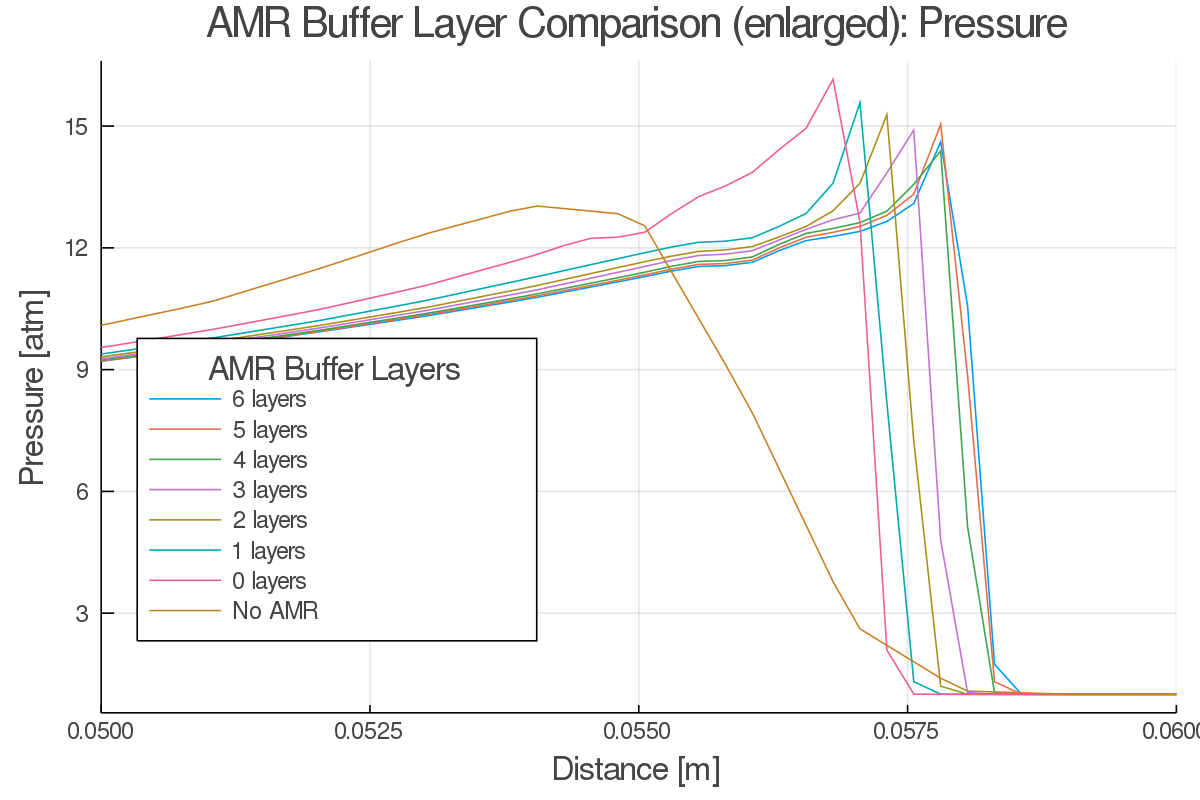
\includegraphics[width=0.8\textwidth]{../figs/amrfigs/amr_bufflayers/pe.png}
\end{center}
\end{frame}

\begin{frame}{AMR Buffer Layer Variation Summary}
\begin{columns}
\column{0.6\textwidth}    
\begin{itemize}
\item 240-40-1 base mesh
\item tracking $||\nabla (p)||$ from 0.2 to 1, unrefining below 0.2, with 3 refinement levels
\item past 4 buffer layers, solution is ``converged''
\item each layer adds around 0.2 mm to wave progression until ``converged'', peak solution largely unchanged
\item cells scale linearly with buffer layers
\end{itemize}
\column{0.4\textwidth}
\begin{table}[h]
\centering
%\caption{Cells for each refinement level for the 250-40-1 simulation at \(t = 3\times 10^{ - 5} s\) in Figure \ref{fig:amr_bufflayers}}
%\label{tab:amr_bufflayers}
\begin{tabular}{cc}
Buffer Layers & Cells \\ \hline
6 & 37,405 \\ 
5 & 34,353 \\
4 & 32,960 \\
3 & 37,678 \\
2 & 16,173 \\
1 & 10,840 \\
None & 10,000 \\
\end{tabular}
\end{table}
\end{columns}
\end{frame}

\subsection{AMR $|| \nabla (p)||$ Refinement Range Variation}

\begin{frame}{AMR $|| \nabla (p)||$ Refine Range Variation: Pressure Distribution}
\begin{center}
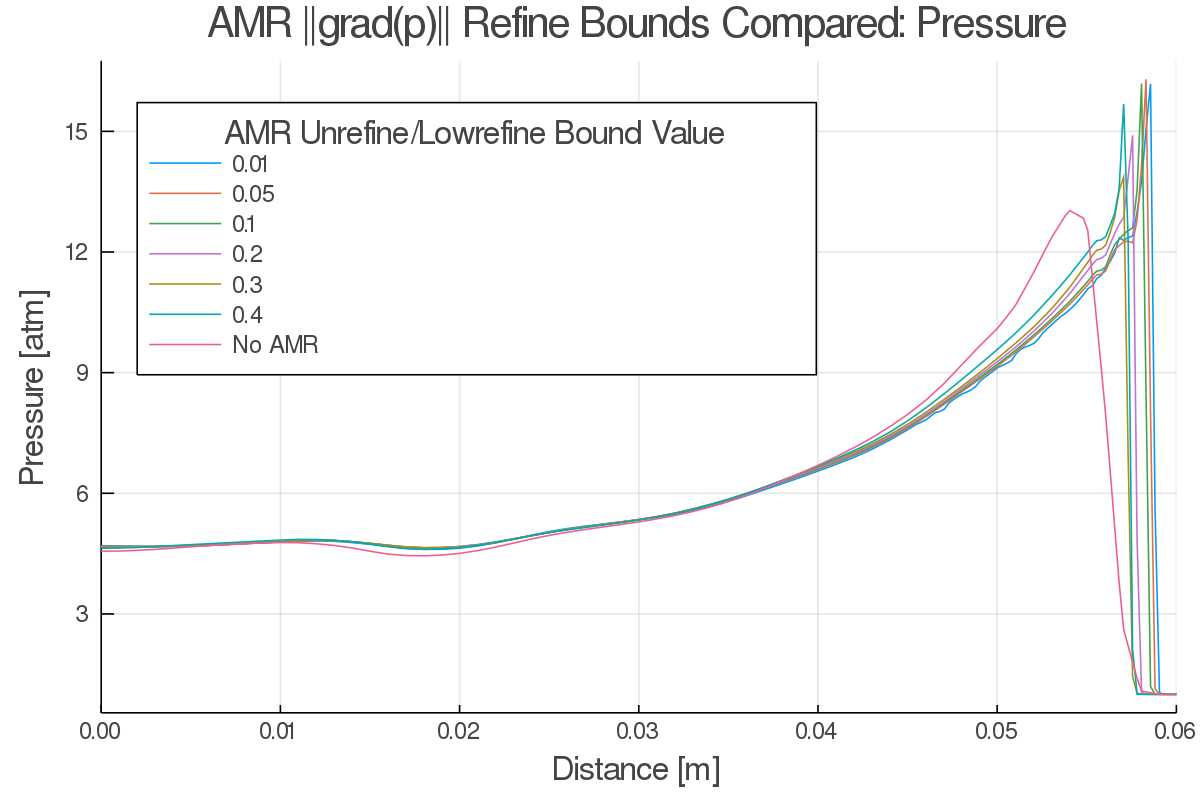
\includegraphics[width=0.8\textwidth]{../figs/amrfigs/amr_refinebounds/p.png}
\end{center}
\end{frame}

\begin{frame}{AMR $|| \nabla (p)||$ Refine Range Variation: Pressure Distribution (enlarged)}
\begin{center}
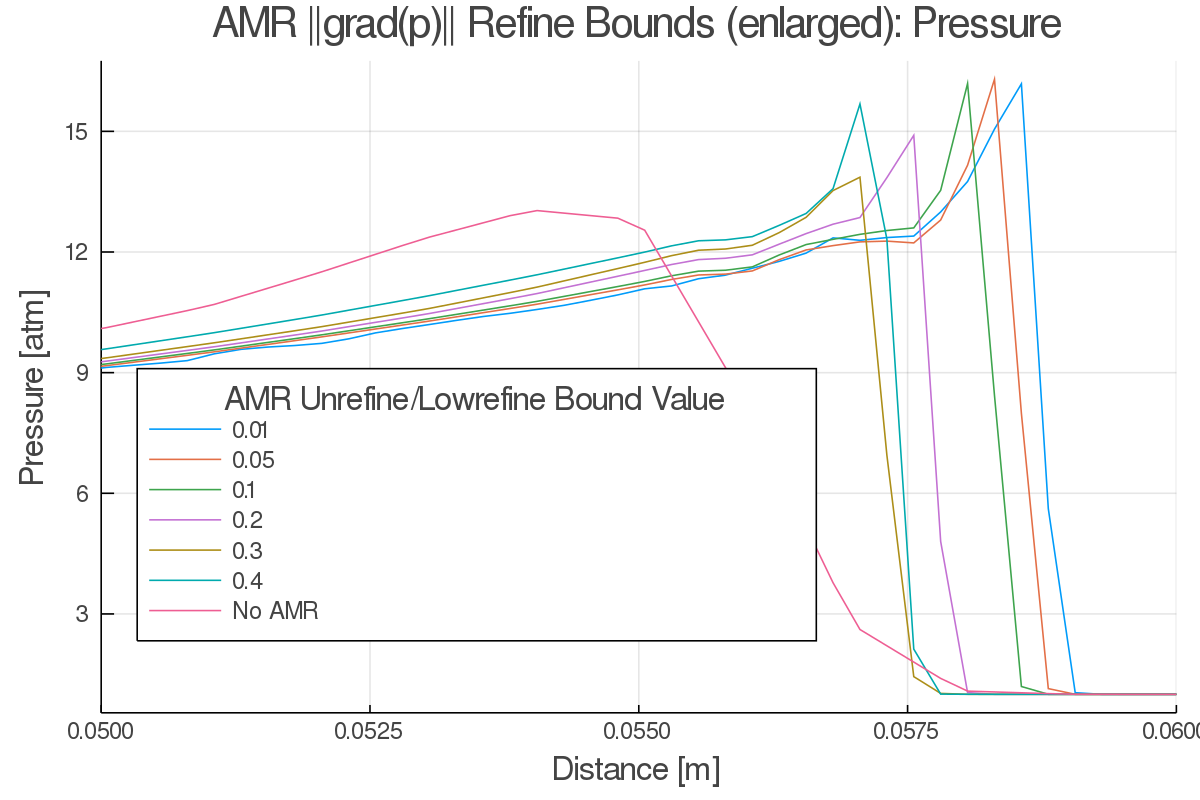
\includegraphics[width=0.8\textwidth]{../figs/amrfigs/amr_refinebounds/pe.png}
\end{center}
\end{frame}

\begin{frame}{AMR $|| \nabla (p)||$ Refinement Range Variation Summary}
\begin{columns}
\column{0.5\textwidth}
\begin{itemize}
    \item 240-40-1 base mesh 
    \item tracking $|| \nabla (p)||$ with 3 refinement and buffer layers
    \item Solution peak values plateau at 0.1 and lower
    \item Below 0.05 computational expense is exponential 
    \item Above 0.05 computational expense is largely unchanged
\end{itemize}

\column{0.5\textwidth}
\begin{table}[h]
\centering
%\caption{Cells for each lower refinement/unrefinement bound for the 250-40-1 simulation at \(t = 3\times 10^{ - 5} s\) in Figure \ref{fig:amr_refinebounds}}
%\label{tab:amr_refinebounds}
\begin{tabular}{cc}
Lower un/refinement bound & Cells \\ \hline
0.01 & 139,136 \\
0.05 & 39,799 \\
0.1 & 38,343 \\ 
0.2 & 37,678 \\
0.3 & 37,692 \\ 
0.4 & 36,355 \\
No AMR & 10,000 \\
\end{tabular}
\end{table}
\end{columns}
\end{frame}

\subsection{Cellular Detonation Modeling}

\begin{frame}{Cellular Detonation Modeling}
\begin{itemize}
\item Cellular ``fishscale'' patterns appear on smoked foils placed in detonation tube experiments
\item Can be used to verify numerical detonation modeling 
\item Numerical simulations can replicate this with maximum pressure and density traces over time for each cell
\item Temperature randomization was seeded throughout the domain, at up to 20\% of the maximum gradient temperature to assist cellular detonation formation 
\end{itemize}
\end{frame}

\begin{frame}{Cellular Detonation Modeling: Initial $T$ Randomization}
\begin{figure}[]
\centering
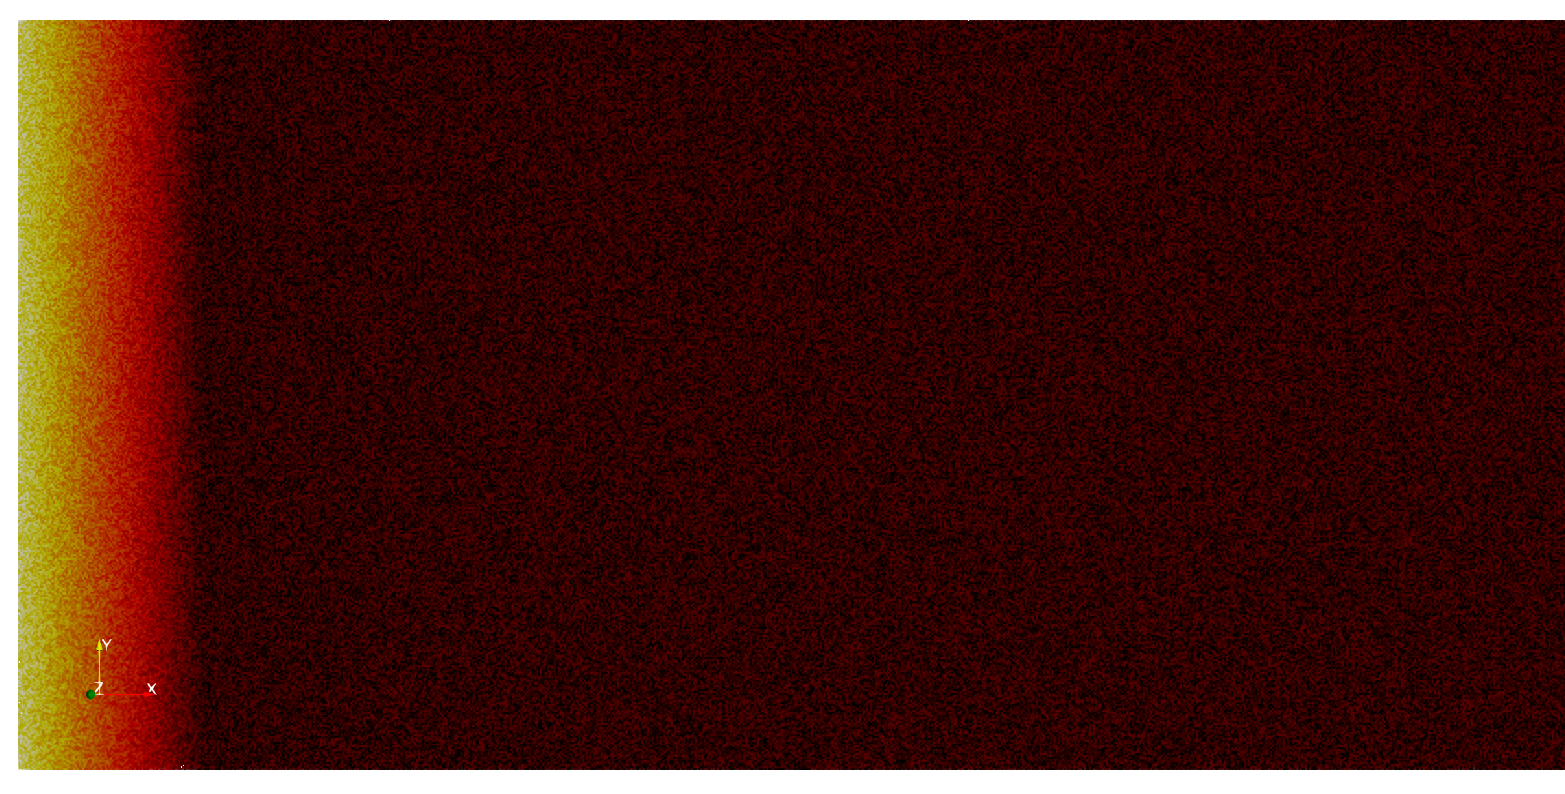
\includegraphics[width=\textwidth]{../figs/ignition/randgrad.png}
%\caption{Gradient ignition method with randomized temperature distribution throughout domain, seen on left side of domain, at t = 0 s}
%\label{fig:gradrand}
\end{figure}
\end{frame}

\begin{frame}{Cellular Detonation Modeling: Maximum $\rho$ Traces}
\begin{figure}[]
\centering
\includegraphics[width=\textwidth]{../figs/example_results/maxrho.png}
%\caption{Surface plot of maximum density tracked across all time steps for each cell, emulating a ``smoke foil''}
%\label{fig:maxrho}
\end{figure}
\end{frame}
